\documentclass[report.tex]{subfiles}
\begin{document}

This chapter presents the data of the experiments described above.
The are later discussed and summarised with relation to the hypotheses in the
following discussion section.
Further information about the system that performed the benchmarks as well as
library versions and experiment code is available in Appendix
\ref{app:experiment}.
\\[0.3cm]

During the evaluation of the parallel model on NEST and BrainScaleS, a
malfunction in PyNN was discovered. 
During the initialisation of the weights PyNN threw an exception in the 
merge layer.
The error was due to the fact that a single population receives weights
from multiple populations, which requires a \textit{view} or a subset of the
population. 
This is done in PyNN using indices, and there is a consistency check to verify
that the index is within a certain range.
Unfortunately the parallel layer requires setting indices out of order, and
the index verification fails.

While all the models compile and passes the structural tests of PyNN,
the experiments using the Merge layer fails to complete.
A complete description of the error trace is available in Section
\ref{lst:pynn_exception} on page \pageref{lst:pynn_exception}.

\section{NAND}
Both the NAND and XOR experiments are built by compiling the expression 
\texttt{\textbf{dense} 2 4 $\obar$ \textbf{dense} 4 2}.
Data from the NAND experiments are shown in Table \ref{tab:xor}.
The rates are below chance level (0.75) in NEST, both during
the random weight initialisation and while transferring weights from Futhark.
However, the accuracy increases significantly when the Futhark weights are
injected.

\def\arraystretch{1.2}
\begin{table}
  \begin{tabular}{r|l l}
  \label{tab:nand}
  Backend & Random weights & Transferred weights \\ \hline
  Futhark & 1 & - \\
  NEST & 0.37 $\pm$ 0.040 & 0.69 $\pm$ 0.216\\ 
  BrainScaleS & N/A & N/A
  \end{tabular}
  \caption{Mean accuracies and standard deviations the NAND experiment.}
  \label{tab:xor}
\end{table}

The error rates plotted in Figure \ref{fig:nand_snn} shows the summed error
rates after each batch.
The plot shows that the errors decreases initially, but begins
to increase after the third batch.
The model with imported weights show a higher accuracy in the beginning, 
but rapidly falls to the same level as the model with randomly initialised
weights.

\begin{figure}
  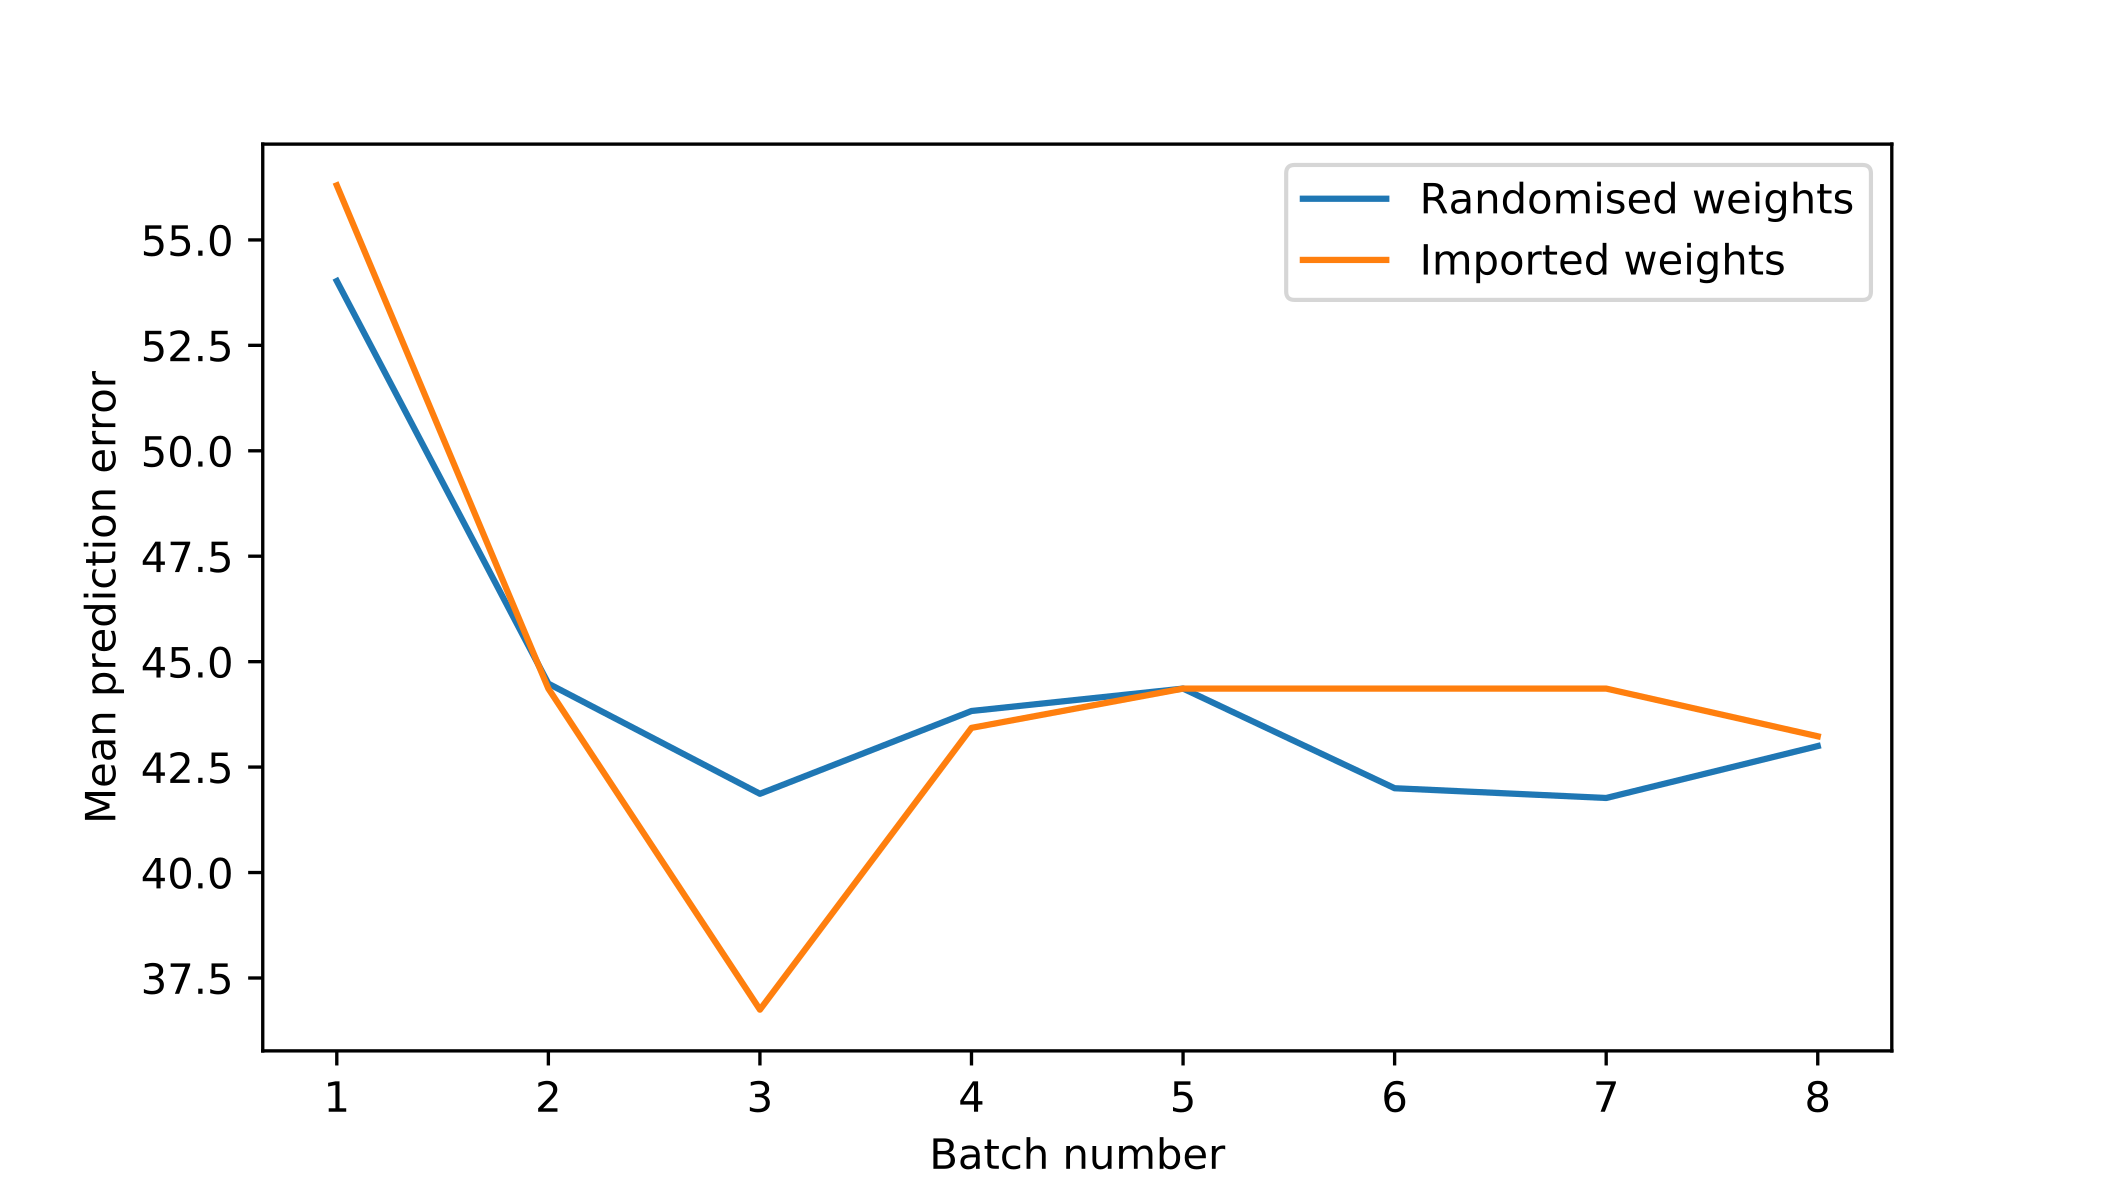
\includegraphics[width=\linewidth]{images/nand.png}
  \caption{Summed gradient error rates for the NAND network simulated in NEST. The rates
  are produced following each batch and are averaged over 10 simulations.}
  \label{fig:nand_snn}
\end{figure}
\FloatBarrier

\section{XOR}

Tabel \ref{tab:nand} shows the XOR experiment results. 
NEST is above chance level (0.5), but with a small margin. The 
weight improvements when transferring the Futhark weights are smaller than 
what was seen in the NAND experiment.

\begin{table}
  \begin{tabular}{r l l}
  Backend & Random weights & Transferred weights \\ \hline
  Futhark & 1.000 & - \\ 
  NEST & 0.530 $\pm$ 0.038 & 0.585 $\pm$ 0.033 \\
  BrainScaleS & N/A & N/A
  \end{tabular}
  \caption{Mean accuracies and standard deviations for the XOR experiment.}
  \label{tab:nand}
\end{table}

The error rates for the XOR network plotted in Figure \ref{fig:xor_snn} shows
the same picture as with the NAND error rates: they decline initially, but grows
after the third batch has been processed.

\begin{figure}
  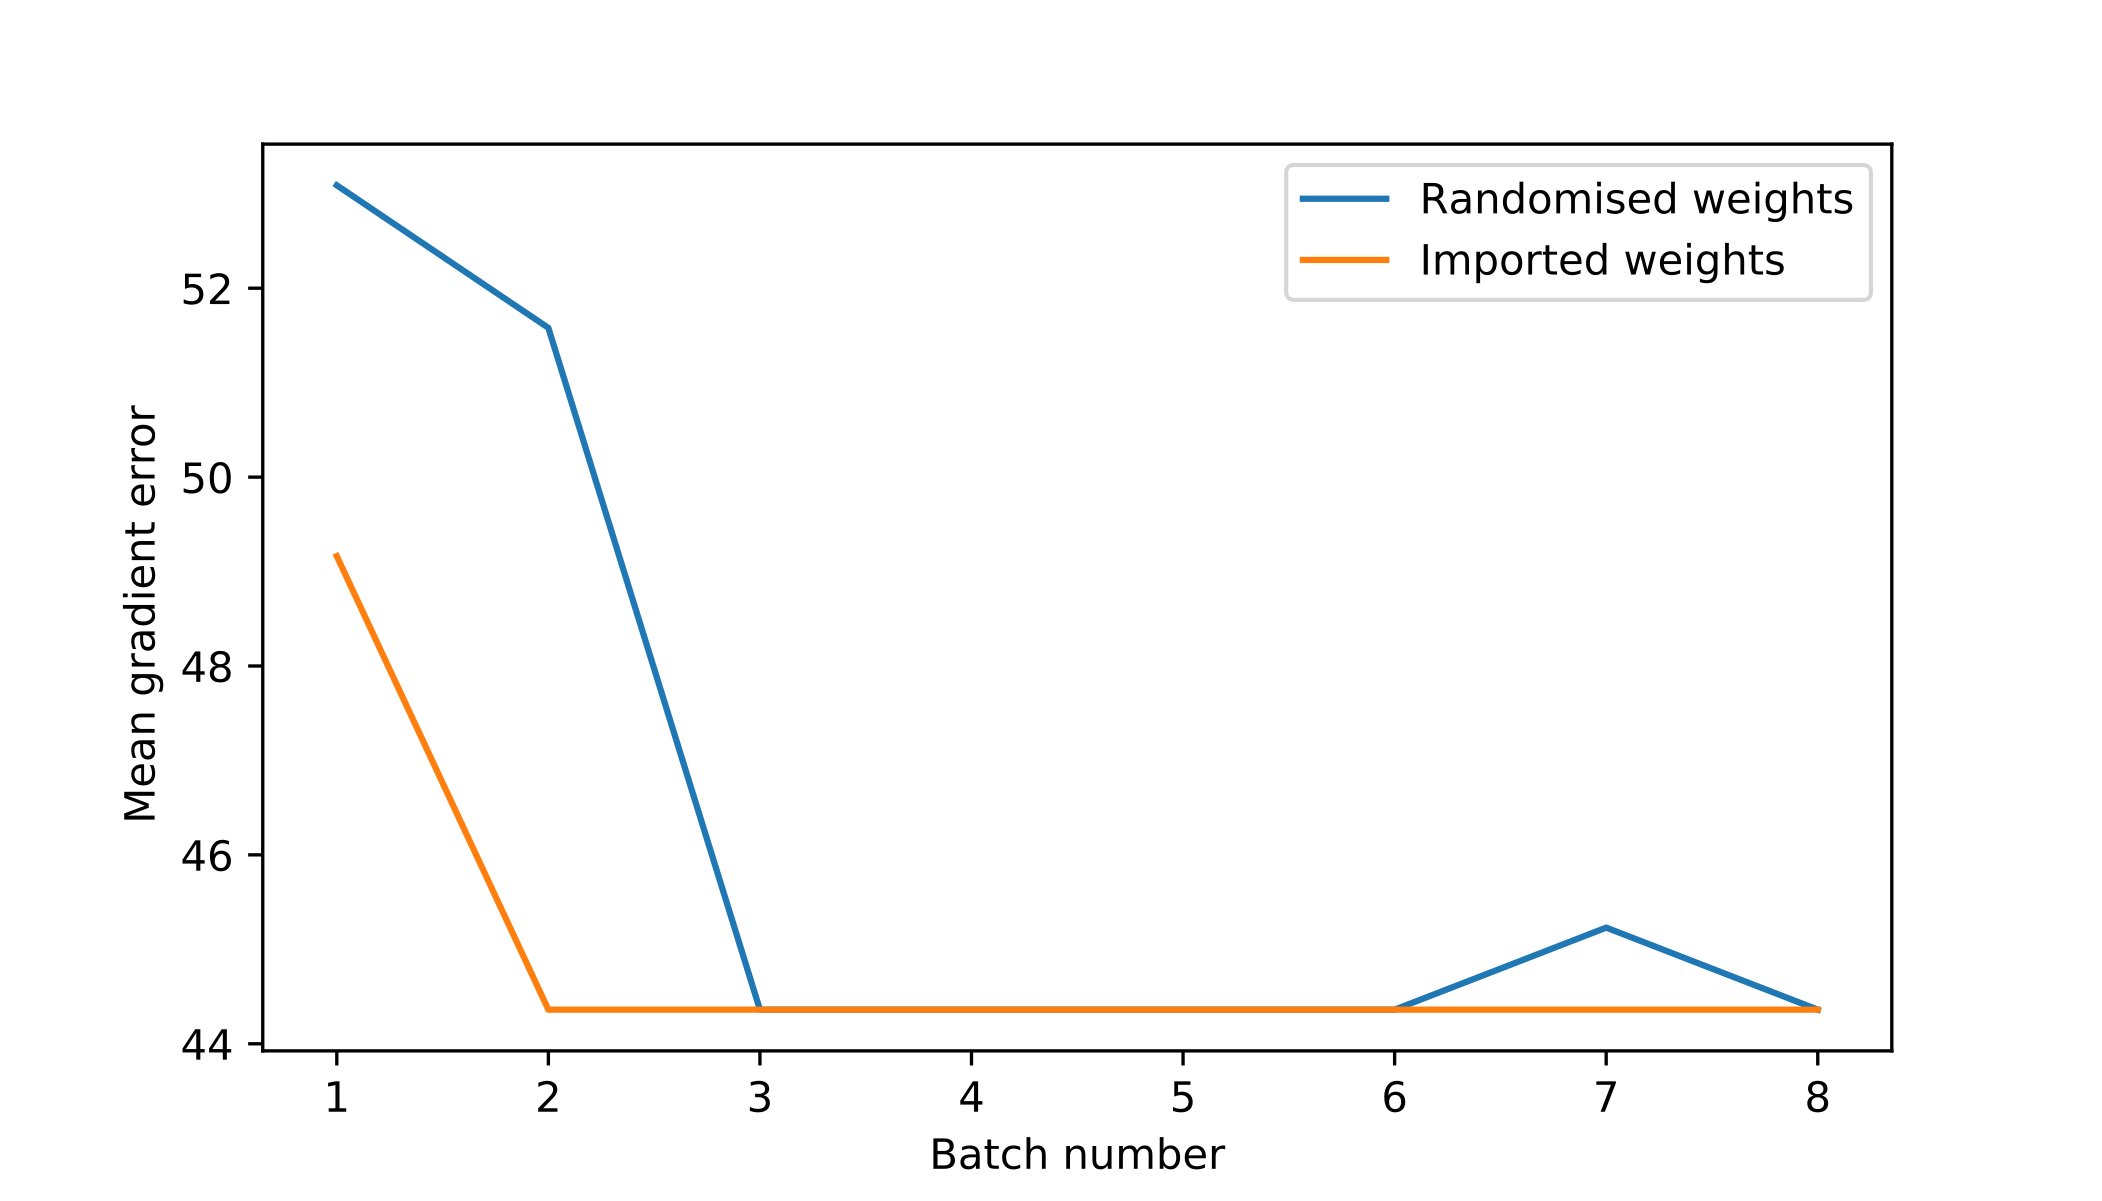
\includegraphics[width=\linewidth]{images/xor.png}
  \caption{Summed error rates for the XOR network simulated in NEST. The rates
  are produced following each batch and are averaged over 10 simulations.}
  \label{fig:xor_snn}
\end{figure}

\FloatBarrier

\section{Sequential MNIST}

Data from Tables \ref{tab:mnist_seq} and\ref{tab:mnist_par} shows the results of
executing the sequential and parallel MNIST experiments.

Futhark performs equally well in the two experiments, but below the
state-of-the-art rates.
NEST performs close to chance level (0.1), with a slight improvement following a
weight transfer.

\begin{table}
  \begin{tabular}{r l l}
  Backend & Random weights & Transferred weights \\ \hline
  Futhark & 0.710 & - \\ 
  NEST & 0.147 $\pm$ 0.044 & $\pm$ \\
  BrainScaleS & N/A & N/A
  \end{tabular}
  \caption{Mean accuracies and standard deviations for the MNIST sequential experiment.}
  \label{tab:mnist_seq}
\end{table}

\begin{table}
  \begin{tabular}{r l l}
  Backend & Random weights & Transferred weights \\ \hline
  Futhark & 0.710 & - \\ 
  NEST & N/A & N/A \\
  BrainScaleS & N/A & N/A
  \end{tabular}
  \caption{Mean accuracies and standard deviations for the MNIST sequential experiment.}
  \label{tab:mnist_par}
\end{table}

\end{document}
